

\begin{figure}[t!]
\begin{center}
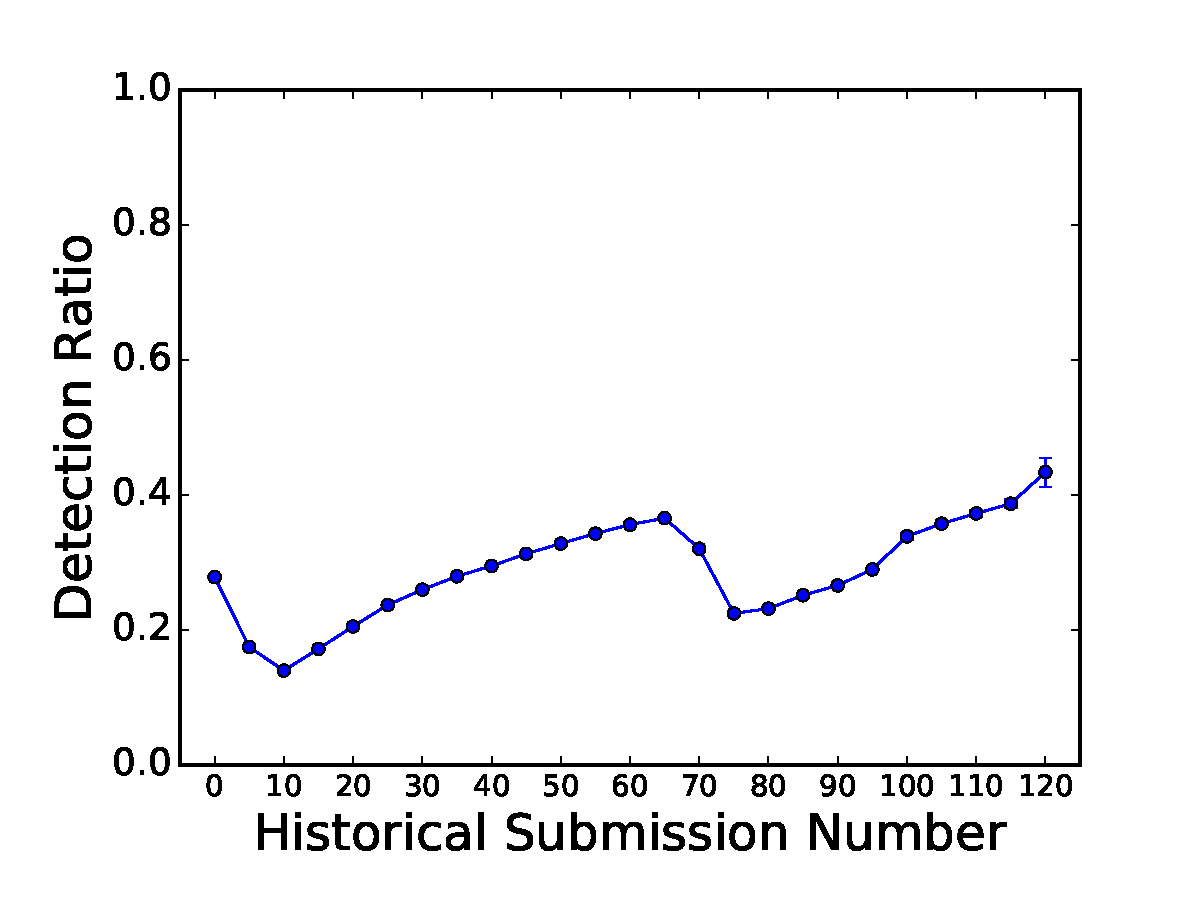
\includegraphics[width=2.5in]{figure/SubNum}
\mycaption{fig:hisnum}{The relation between historical submission number and detection rate.}
{
How detection rate changes with historical submission number (rounded up to nearest 5).
95\% confidence interval is also drawn for each point.   
}
\end{center}
%\vspace{-0.25in}
\end{figure}

\begin{figure}[t!]
\begin{center}
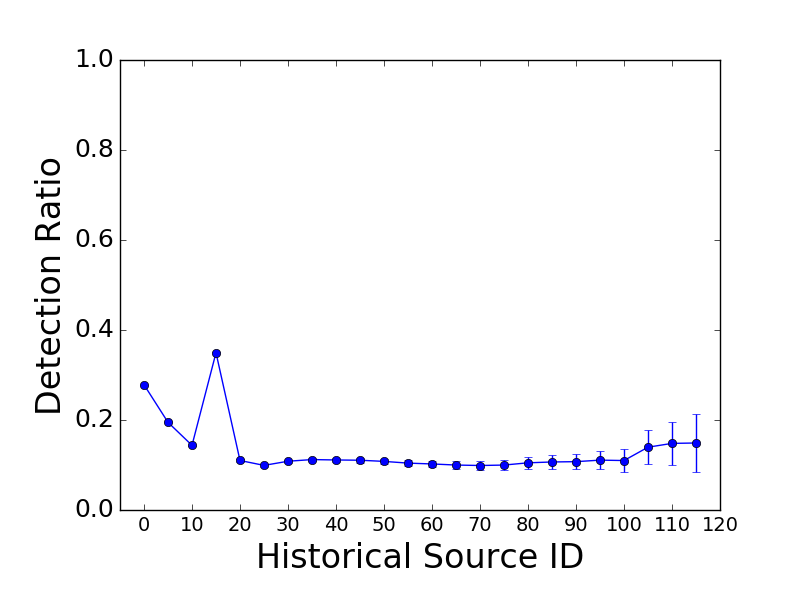
\includegraphics[width=2.5in]{figure/SubID}
\mycaption{fig:hisid}{The relation between the number of previous source ids and detection rate.}
{
How detection rate changes with the number of historical source id (rounded up to nearest 5).
95\% confidence interval is also drawn for each point.   
}
\end{center}
%\vspace{-0.25in}
\end{figure}

\begin{figure}[t!]
\begin{center}
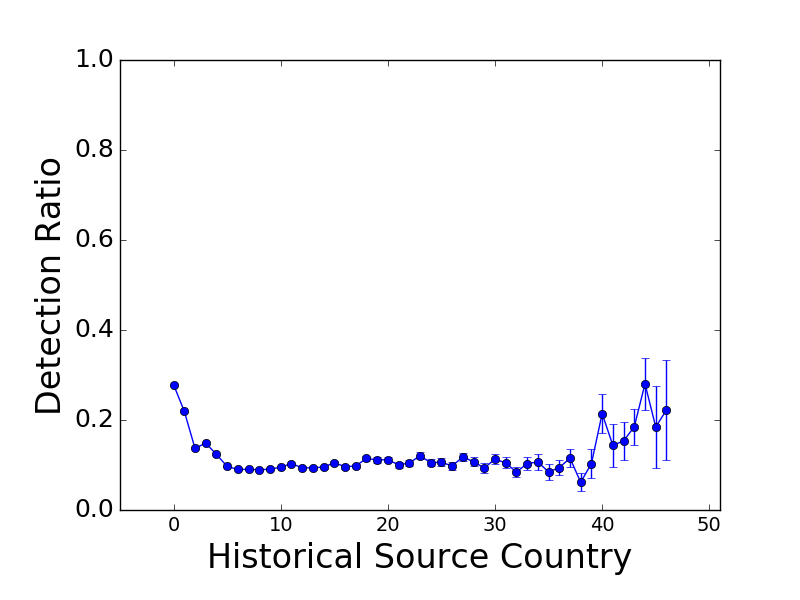
\includegraphics[width=2.5in]{figure/SubCountry}
\mycaption{fig:hisid}{The relation between the number of previous source countries and detection rate.}
{
How detection rate changes with the number of historical source countries.
95\% confidence interval is also drawn for each point.   
}
\end{center}
%\vspace{-0.25in}
\end{figure}
